% =====================================================================
% Slide 9: Stage 3 -- Quantum Espresso DFT references
% =====================================================================
\begin{frame}{Stage 3: Quantum Espresso DFT References}
\begin{columns}[T]
\column{0.45\textwidth}
\centering
\scriptsize
\setlength{\tabcolsep}{4pt}
\renewcommand{\arraystretch}{0.95}
\begin{tabular}{llrrr}
\toprule
Element & Lat. & $a_{0}$ (\AA) & $E_{\mathrm{coh}}$ & $B$ (GPa) \\
\midrule
Al & FCC     & 4.047 & 3.611 &  77.5 \\
Cu & FCC     & 3.639 & 3.857 & 138.5 \\
Si & DIAMOND & 5.471 & 5.130 &  89.3 \\
Ti & HCP     & 2.915 & 6.284 & 114.5 \\
Zn & HCP     & 2.766 & 0.964 &  68.4 \\
Cr & BCC     & 2.848 & 3.964 & 213.1 \\
Fe & BCC     & 2.806 & 6.834 & 420.5 \\
Mg & HCP     & 3.177 & 1.483 &  47.8 \\
Mn & BCC     & 2.803 & 3.728 & 225.7 \\
Mo & BCC     & 3.169 &10.353 & 280.8 \\
\bottomrule
\end{tabular}\\[0.2em]
\textit{Elemental references}
($E_{\mathrm{coh}}$ in eV/atom; Birch--Murnaghan fits).

\column{0.54\textwidth}
\centering
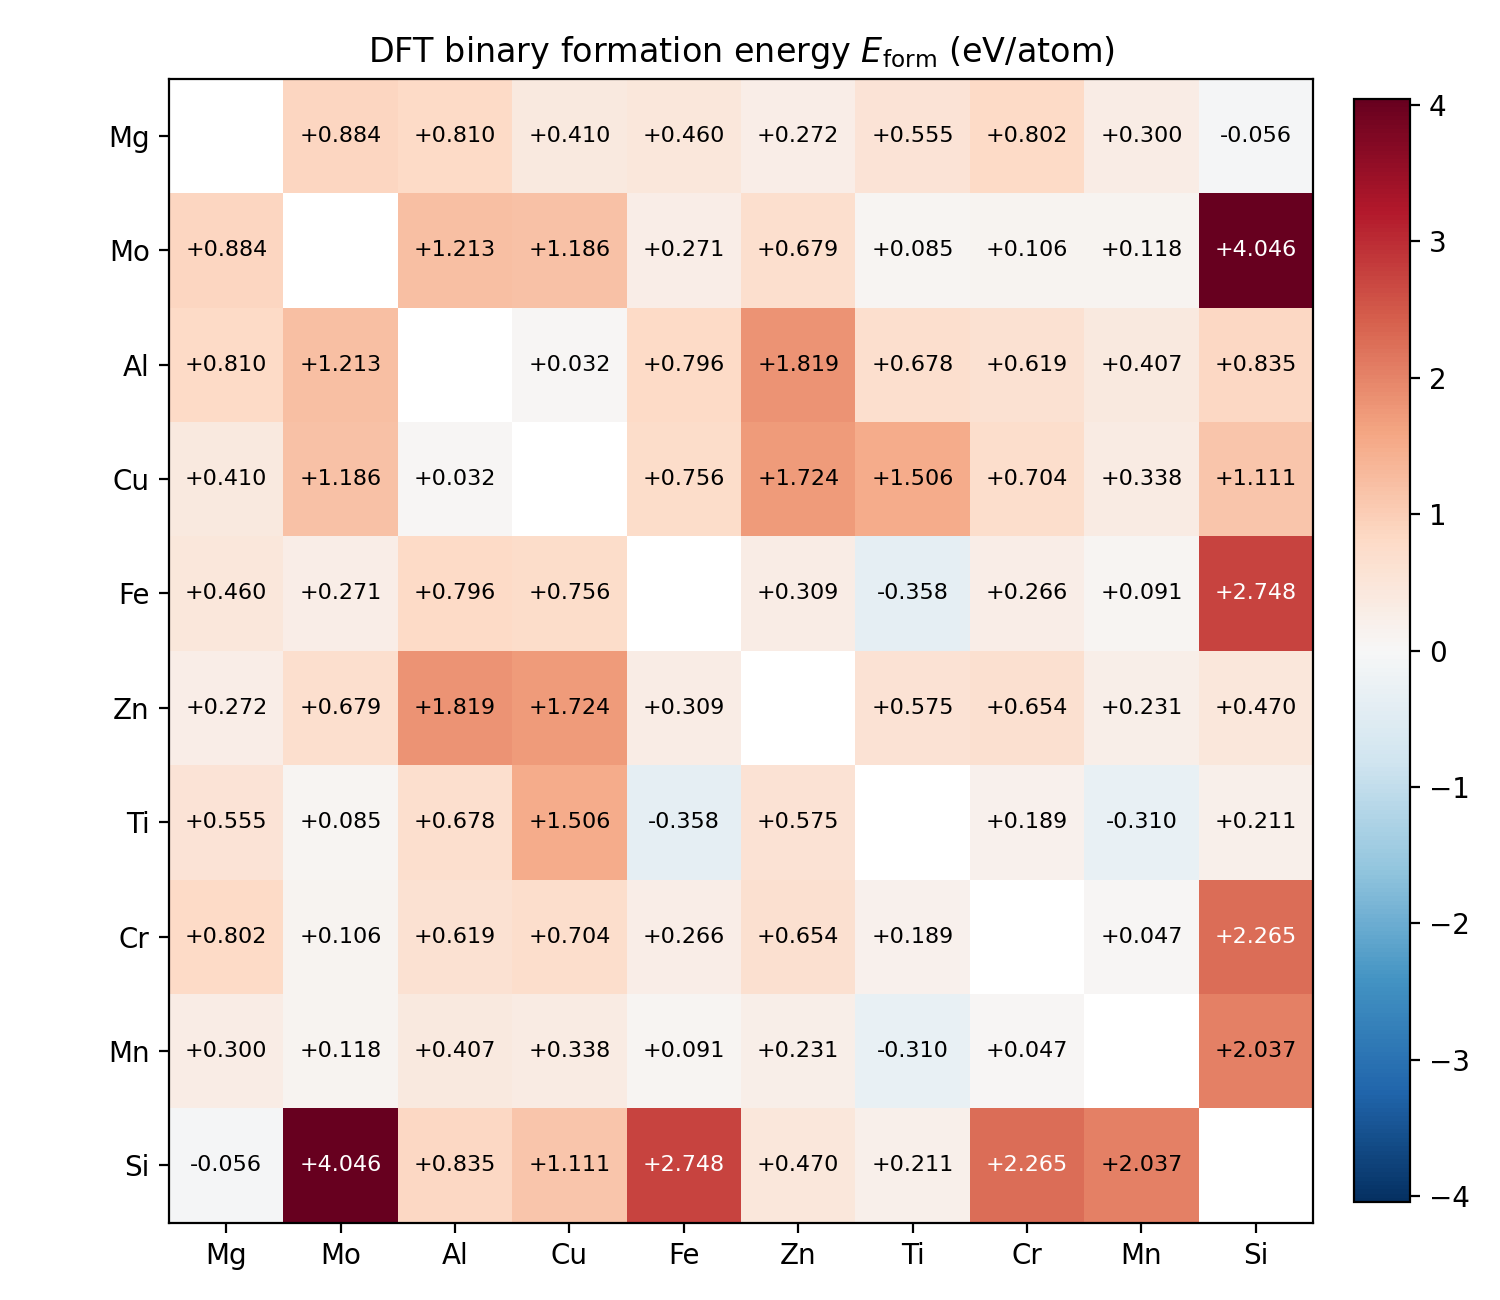
\includegraphics[height=5.7cm,keepaspectratio]{figures/formation_energy_heatmap.png}\\[-0.25em]
\scriptsize Binary formation energies $E_{\mathrm{form}}(i, j)$
(eV/atom). Negative values indicate exothermic mixing; positive
values indicate limited mutual solubility. These references seed
the MEAM cross-term parameters.
\end{columns}
\end{frame}
